%%==================================================================%%
%% Author : P�rez Ruiz, Alejandro                                   %%
%% Author : S�nchez Barreiro, Pablo                                 %%
%% Version: 1.1, 16/03/2011                                         %%                                                                                    %%                                                                  %%
%% Memoria del Proyecto Fin de Carrera                              %%
%% DomainEngineering/Arcchitecture                                  %%
%%==================================================================%%

El hogar inteligente posee una serie de dispositivos que se descomponen en sensores y actuadores. Los sensores son los encargados de obtener ciertos datos, como por ejemplo, los grados que hace en una habitaci�n o la apertura que tiene una ventana. Los actuadores se encargan de ejecutar las ordenes, por ejemplo, de que una persiana se abra o se cierre o de que la calefacci�n se encienda a unos determinados grados.

Tanto los sensores como los actuadores se encuentran conectados a un dispositivo central que los coordina, el cual se conoce como puerta de enlace o Gateway. Dicho Gateway se encarga de recibir los datos de los sensores, procesarlos y enviar las ordenes adecuadas a los actuadores. De igual modo, el Gateway recibe �rdenes de los usuarios que son ejecutadas por los actuadores para modificar los elementos de la casa.

Adem�s el Gateway posee una lista de las plantas que tiene el hogar, a su vez cada planta contiene otra lista de las habitaciones que se encuentran en dicha planta, y un objeto tiempo que se encarga de simular el transcurso del tiempo en el sistema.

En la figura \ref{domain:fig:defArq} se puede observar el dise�o UML que representa todo lo dicho anteriormente, quedando reflejado como el Gateway es la pieza central del sistema.

\begin{figure}[!tb]
 \centering
 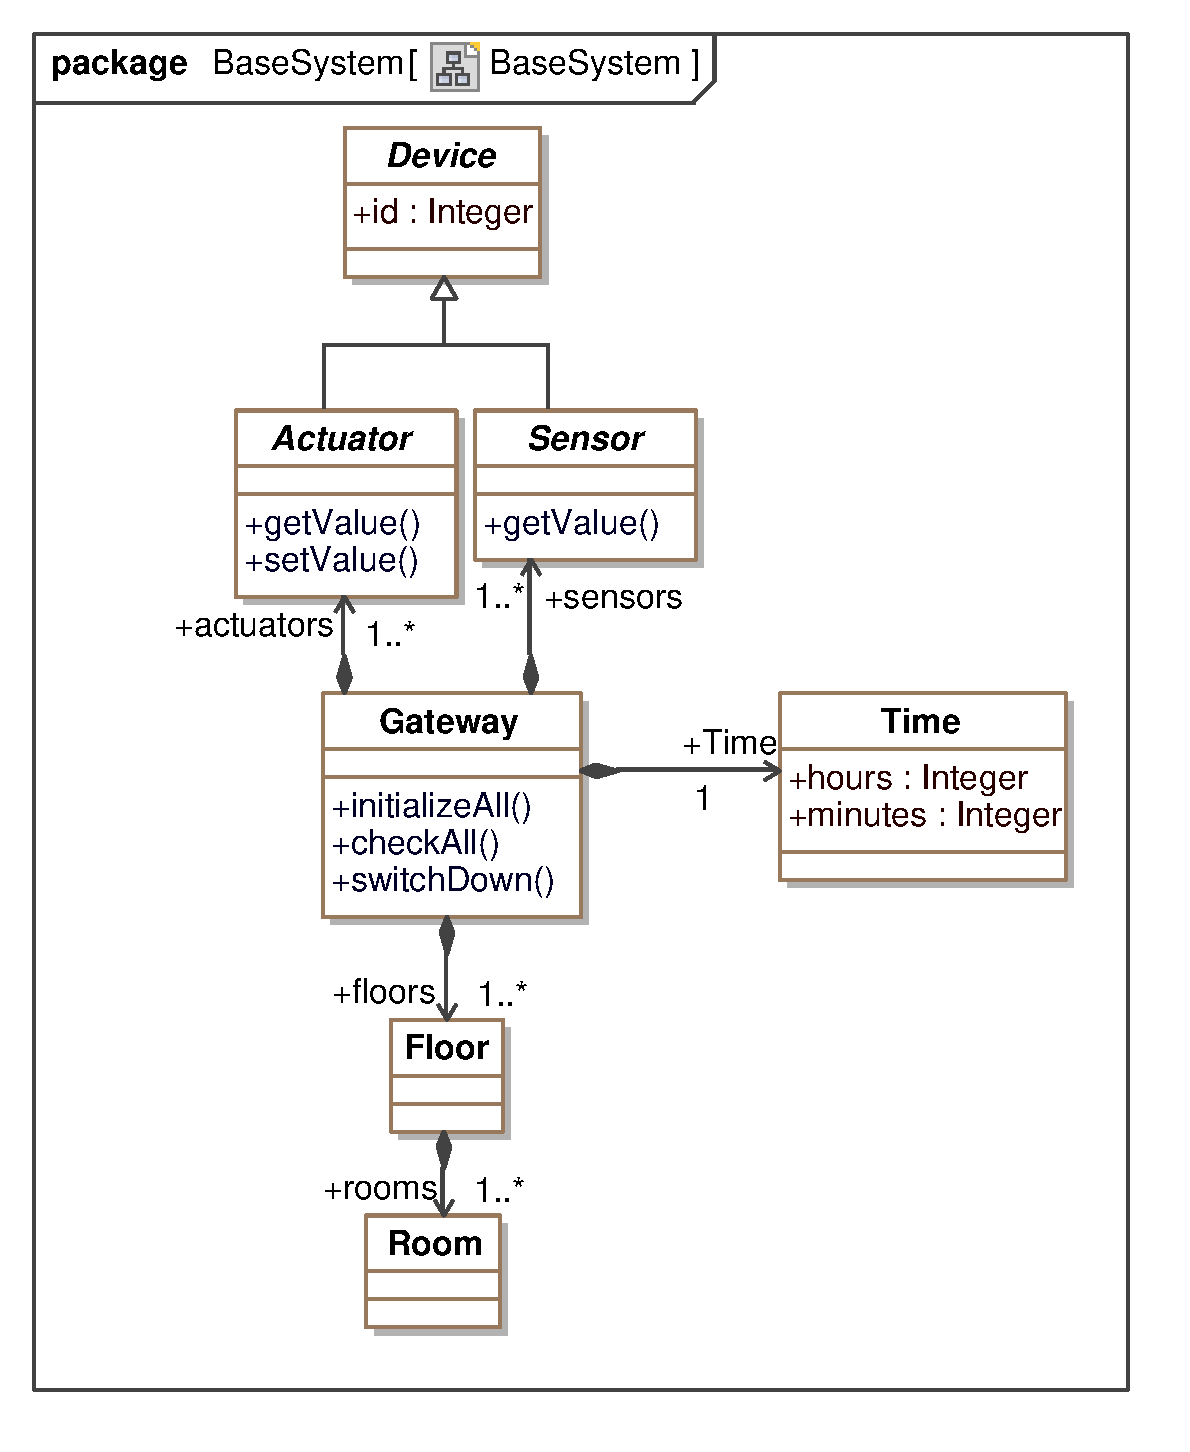
\includegraphics[width=.45\linewidth]{domainEngineering/Images/definicionArq.eps} \\
 \caption{Dise�o UML que muestra la definici�n arquitect�nica}
 \label{domain:fig:defArq}
\end{figure}

Para que el usuario pueda monitorizar y controlar la situaci�n de los elementos es necesario la creaci�n de una interfaz gr�fica que represente las funcionalidades propias del Gateway. De igual modo, es necesaria otra interfaz gr�fica que juegue el papel de simulador, ya que la implementaci�n presentada en este proyecto no est� conectada a dispositivos reales, y por ello es necesario simular valores para los sensores, tales como la temperatura, y el tiempo del sistema. Ambas interfaces gr�ficas se conectar�n al Gateway para poder comunicarse con todos los dispositivos.

Debido a que el Gateway simplifica la comunicaci�n entre los objetos del sistema siendo �ste un objeto que gestiona la distribuci�n de mensajes entre sensores, actuadores, e interfaces gr�ficas, se puede decir que sigue el patr�n de dise�o denominado \emph{mediador}\cite{gamma:1994} (\emph{Mediator pattern}, en ingl�s).

En el dise�o arquitect�nico descrito anteriormente se observa que existen dependencias entre objetos de forma que cuando un objeto cambia de estado, todos sus objetos dependientes son notificados y actualizados. Tales dependencias son:
\begin{enumerate}
\item Las interfaces gr�ficas y el Gateway tienen que ser notificados y actualizados cada vez que un sensor cambie.
\item Tanto el Gateway como las interfaces gr�ficas tienen que ser actualizados cuando el tiempo actual del sistema cambie.
\end{enumerate}
Claramente esto puede ser modelado siguiendo el patr�n de dise�o llamado \emph{observador}\cite{gamma:1994} (\emph{Observer pattern}, en ingl�s), es decir, por cada objeto que vaya a ser observado es necesario crear una lista donde se registrar�n todos los observadores, de este modo cada vez que se produzca una modificaci�n en el objeto observado, �ste utilizar� la lista para notificar a todos sus observadores que se ha producido un cambio.

Con el dise�o arquitect�nico b�sico definido y teniendo en cuenta que el presente proyecto implementa una l�nea de productos software para hogares inteligentes, se debe encapsular cada una de las caracter�sticas ,para que posteriormente cada aplicaci�n creada pueda ser compuesta de diferentes maneras. Por ello se har� uso de las clases parciales y la herencia para encapsular cada caracter�stica. Este proceso iterativo ser� descrito con mas detalle en las siguientes secciones.
